\documentclass{article}
\usepackage[utf8]{inputenc}
\usepackage[margin=1in]{geometry}
\usepackage{amsmath}
\usepackage{tikz}
\usepackage{tikz-dimline}
\usepackage{hyperref}

\usetikzlibrary{calc}
\tikzset{no slope/.code={\pgfslopedattimefalse}}

\hypersetup{
    colorlinks=true,
    linkcolor=blue,
    filecolor=magenta,      
    urlcolor=cyan,
}

\newcommand{\rlpr}[1]{\left(#1\right)}
\newcommand{\rlvc}[1]{\left\langle#1\right\rangle}
\newcommand{\rlabs}[1]{\left|#1\right|}

\title{Finding the $h$ Parameter of a Ray-Ellipse Interaction}
\author{Ryan Lefkowitz}
\date{November 15, 2019}

\begin{document}

\maketitle

\section{Determining $h$}

\noindent Given an ellipse centered at the origin with major and minor axes $a$ and $b$ defined by
\begin{equation}
    \frac{x^2}{a^2} + \frac{y^2}{b^2} = 1
\end{equation}
and a ray with origin $\vec{o} = \rlvc{o_x, o_y}$ and direction $\vec{d} = \rlvc{d_x, d_y}$, the parameter $h$ for the intersection of the ray and ellipse can be computed as:
\begin{equation}
    h = \rlabs{\frac{m}{n}}\text{, where }m = \vec{o}\cdot\rlvc{-d_y, d_x}\text{ and }n =\vec{p}\cdot\rlvc{-d_y, d_x}
\end{equation}
where $\vec{p}$ is a point on the ellipse at which the tangent vector is parallel to $\vec{d}$.
\begin{center}
    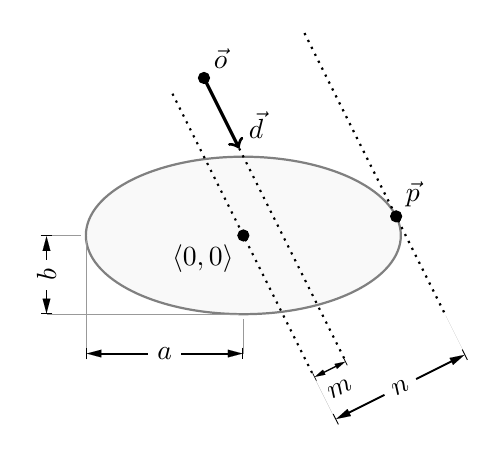
\begin{tikzpicture}
    
        % general coordinates
        \coordinate (origin) at (0,0);
        
        % ray coordinates
        \coordinate (ray-origin) at (-0.5, 2);
        \coordinate (ray-direction) at (0.447213595,-0.894427191);
        \coordinate (ray-direction-location) at ($(ray-origin) + (ray-direction)$);
        
        % ellipse coordinates
        \coordinate (top) at (0,1);
        \coordinate (right) at (2,0);
        \coordinate (bottom) at (0,-1);
        \coordinate (left) at (-2,0);
        
        % draw ellipse
        \filldraw[color=gray,fill=gray!5, thick] (0,0) ellipse (2 and 1);
        \draw node (A) at (-2, -1.5) {};
        \dimline[line style = {line width=0.70},
                 label style = {no slope},
                 extension start path={(A) ($(left) + (0,-0.06)$)},
                 extension end path={($(A) + (2, 0)$) ($(bottom) + (0,-0.06)$)}] {(A)}{($ (A) + (2,0) $)}{$a$};
        \draw node (A) at (-2.5, -1) {};
        \dimline[line style = {line width=0.70},
                 extension start path={(A) ($(bottom) + (-0.06,0)$)},
                 extension end path={($(A) + (0, 1)$) ($(left) + (-0.06,0)$)}] {(A)}{($ (A) + (0,1) $)}{$b$};
        
        % draw origin
        \filldraw[black] (origin) circle (2pt) node[anchor=north east] {$\langle0,0\rangle$};
        
        % draw ray
        \filldraw[black] (ray-origin) circle (2pt) node[anchor=south west] {$\vec{o}$};
        \draw[->, very thick] (ray-origin) -- (ray-direction-location);
        \filldraw[black] (ray-direction-location) circle (0pt) node[anchor=south west] {$\vec{d}$};
        
        % draw ray extension
        \draw[dotted, thick] (ray-direction-location) -- ($(ray-origin) + 2*2.01246118*(ray-direction)$);
        
        % draw origin extension
        \draw[dotted, thick] ($(origin) - 2.01246118*(ray-direction)$) -- ($(origin) + 2.01246118*(ray-direction)$);
        
        % draw tangent
        \coordinate (tangent-point) at (1.94028500045,0.242535624717);
        \filldraw[black] (tangent-point) circle (2pt) node[anchor=south west] {$\vec{p}$};
        \draw[dotted, thick] ($(tangent-point) + 1.36166981*(ray-direction)$) -- ($(tangent-point) - 2.66325255*(ray-direction)$);
        
        % draw measurements
        \coordinate (tangent-line-end) at ($(tangent-point) + 1.36166981*(ray-direction)$);
        \coordinate (origin-line-end) at ($(origin) + 2.01246118*(ray-direction)$);
        \coordinate (ray-line-end) at ($(ray-origin) + 2*2.01246118*(ray-direction)$);
        \dimline[label style={below=0.5ex},
                 line style = {line width=0.50},
                 extension start length = 0,
                 extension end length = 0] {(origin-line-end)}{(ray-line-end)}{$m$};
        \dimline[line style = {line width=0.70},
                 extension start length = -0.3,
                 extension end length = -0.3] {($(origin-line-end) + 0.6*(ray-direction)$)}{($(tangent-line-end) + 0.6*(ray-direction)$)}{$n$};
        
    \end{tikzpicture}
\end{center}

\subsection{Determining $\vec{p}$}


Given a point $(x, y)$ on the ellipse, the normalized tangent vector $\vec{t}$ can be computed as:
\begin{equation}
    \vec{t} = \frac{\rlvc{ ya^2, -xb^2 }}{\sqrt{x^2 b^4 + y^2 a^4}}.
\end{equation}
Solving for $x$ and $y$, it can be determined that
\begin{equation}
    \vec{p} = c\cdot\rlvc{ -a^2 d_y, b^2 d_x } \text{, where } c = \sqrt{\frac{1}{a^2 d_y^2 + b^2 d_x^2}}.
\end{equation}
Substituting the value of $\vec{p}$ in Equation 2 yields:
\begin{equation}
    h = \rlabs{\frac{o_y d_x - o_x d_y}{\sqrt{a^2 d_y^2 + b^2 d_x^2}}}.
\end{equation}
An interactive tool can be found at \url{https://www.desmos.com/calculator/m1vsowmkvi}


\end{document}

